%!TEX root = ../thesis.tex

\chapter{Umsetzung}
\label{chap:umsetzung}

Im Nachfolgenden soll die Konzeption und Umsetzung der in \ref{sec:anforderungsanalyse}
beschriebenen Anforderungen an das Projekt \projectname{} erläutert werden.
Der Schwerpunkt soll dabei speziell auf die Cross Plattform Architektur sowie auf die
Entwicklung der Komponenten hinsichtlich Wiederverwendbarkeit gerichtet werden.


\section{Applikationsstruktur}

Dieses Kapitel beschäftigt sich mit der Konzeptphase der Plattformübergreifenden Applikationsstruktur
(Abbildung \ref{kapitel4/arch}).
Um Endprodukte für Web, Desktop und App zu generieren, werden die Frameworks Angular 2, Electron und das
Ionic \ac{SDK} verwendet. Die Codebase für die Web- und Desktop Anwendungen lassen sich so weit vereinen,
dass diese innerhalb eines Repositories implementiert werden können.
Ein weiteres Repository beinhaltet die hybride Applikation,
welche mithilfe des Ionic 2 \ac{SDK} entwickelt wird. Obwohl Ionic 2 auf das Angular Framework aufbaut,
macht es Sinn den Web und App Code voneinander getrennt zu behandeln.
Gründe dafür sind zum einen konzeptionelle Unterschiede im Aufbau der Applikation
sowie unterschiedliche Navigation APIs der Frameworks.
Die \ac{UI} und Funktionalität wird daher innerhalb der Angular 2
Anwendung in Form von wiederverwendbaren Komponenten entwickelt und
Repository-übergreifend für die Verwendung im Ionic 2 Projekt verteilt.

\begin{itemize}
  \item Angular 2/Web und Desktop: github.com/michaelknoch/mia
  \item Ionic 2/App: github.com/michaelknoch/miamobile
\end{itemize}



\begin{figure}[h]
 \centering
 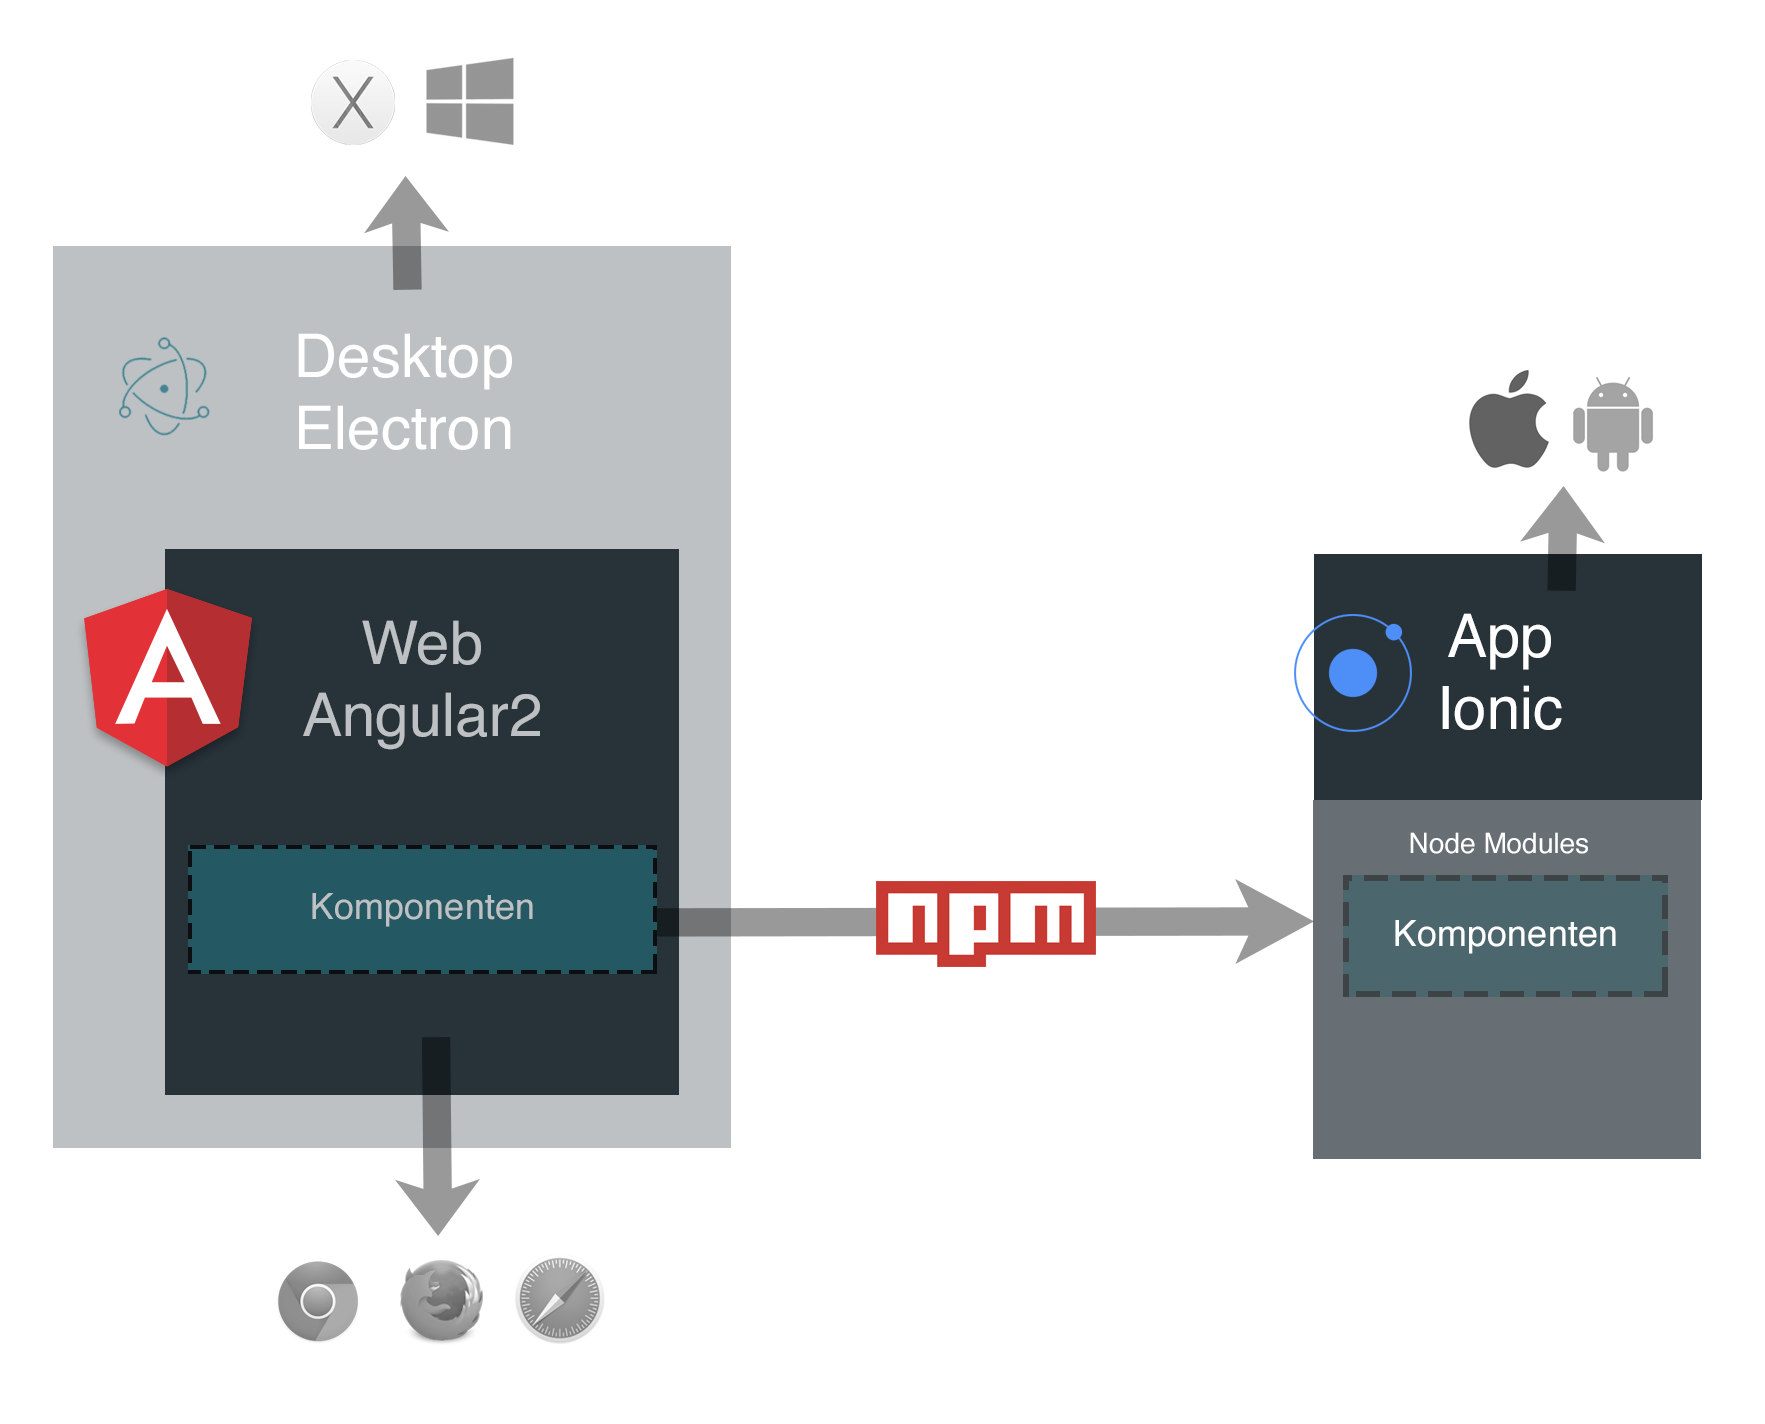
\includegraphics[width=\linewidth]{kapitel4/arch.png}
 \caption{Cross Plattform Architektur}
 \label{kapitel4/arch}
\end{figure}
\vspace{0.3cm}



\section{Komponentenentwicklung}

\subsection{Komponententypen}

Im Folgenden werden Ansätze der Komponentenentwicklung bezüglich der in
\projectname{} erforderlichen Funktionalitäten entwickelt.


\subsubsection{generischer Ansatz}

Bei der Entwicklung generischer Komponenten ist der Begriff der Wiederverwendbarkeit von zentraler Bedeutung.
Komponenten werden gegenüber dem spezifischen Ansatz nicht für einen definierten Anwendungsfall konzipiert,
sondern können
für diverse, womöglich ähnliche Anwendungsbereiche genutzt werden.
Typisch für generische Angular 2 Komponenten ist die Verwendung des @Input Kanals.
Dabei werden zum einen Daten- sowie Konfigurationsobjekte von außen in die Komponente eingeschleust.
Anhand der Konfigurationsobjekte können generische Komponenten individuell an verschiedene Bedürfnisse angepasst werden.
Durch den Transfer von Datenobjekten wird der Vorgang der Aggregation aus der Komponente abstrahiert und es werden eventuelle
Abhängigkeiten zu Services oder API-Servern vermieden.

Komponenten,
die anhand des generischen Ansatzes entwickelt werden,
sollen nicht nur in der mobilen Ionic App,
sondern projektübergreifend Verwendung finden.
Daher wurde ein Teil der in \projectname{} entwickelten Komponenten anhand des generischen Ansatzes
entwickelt und Open Source auf Github veröffentlicht.
Dadurch können diese von Dritten genutzt und bei Bedarf um Funktionalität erweitert werden.


\subsubsection{spezifischer Ansatz}

Einige Komponenten lassen sich aufgrund ihrer spezifischen Funktionalität nicht generisch entwickeln.
Da sie nur einen spezifischen Anwendungsfall abdecken, können sie nur schwer in anderen Projekten wiederverwendet werden.
Dennoch werden diese innerhalb des Projekts \projectname{}
in der Angular 2 sowie in der Ionic 2 Anwendung verwendet.
Beispiele für spezifische Komponenten sind View- und Menükomponenten welche die Grundstruktur einer Applikation abbilden.

\subsection{MVC und Abhängigkeiten}

Im Idealfall können Komponenten voneinander gekapselt entwickelt werden,
sodass sie völlig eigenständig nutzbar sind und untereinander keine Abhängigkeiten aufweisen.
Jede Komponente beinhaltet individuelle \ac{MVC} Schichten für die Implementierung der Funktionalität von der View bis zur Datenschicht.
Modelklassen (Typisierung) und Services befinden sich innerhalb der Komponente und nicht innerhalb eines globalen Model Layers.
Allerdings entstehen im Aufbau einer Angular Applikation schnell komponentenübergreifende Abhängigkeiten.
Wird Funktionalität in Services, welche von mehreren Komponenten genutzt wird, implementiert
so sollte diese nicht in die Komponente gekapselt werden, sondern sich in einer sichtbaren Schicht zur globalen Verwendung befinden.
Ferner ist es warscheinlich, dass Typescript Modelklassen (Typisierung) ebenfalls in mehreren Komponenten verwendet werden.
Dennoch sollten diese nicht redundant implementiert,
sondern zentral zur Verfügung gestellt werden. Es stellt sich also heraus,
dass nicht alle Komponenten der Applikation \projectname{} als eigenständige Module ausgeliefert werden können,
sondern es durchaus Sinn ergibt, Komponentenpakete über die Infrastruktur zu verteilen.


\subsection{Komponenten Generator}

Um den Entwicklungsprozess der Anwendung zu beschleunigen, wurde mithilfe von \emph{yeoman.io} ein Komponenten-Generator entwickelt.
Dieser ermöglicht es die Grundstruktur neuer Komponenten anhand diverser Optionen in kurzer Zeit auszuliefern.
Dabei wird der Name sowie der Auslieferungsort der neuen Komponente während der Generierung im Terminal erfragt.
Zusätzlich kann definiert werden, ob externe \ac{HTML} und \ac{CSS} Dateien angelegt, oder ob diese inline in der Komponente genutzt werden sollen.
Der Generator wurde ebenfalls Open Source entwickelt und auf Github veröffentlicht
(github.com/michaelknoch/generator-ng2-comp).

\section{Implementierung}


\subsection{Login und Authentifikation}
\label{Login-und-Authentifikation}

\begin{figure}[hptb]
 \centering
 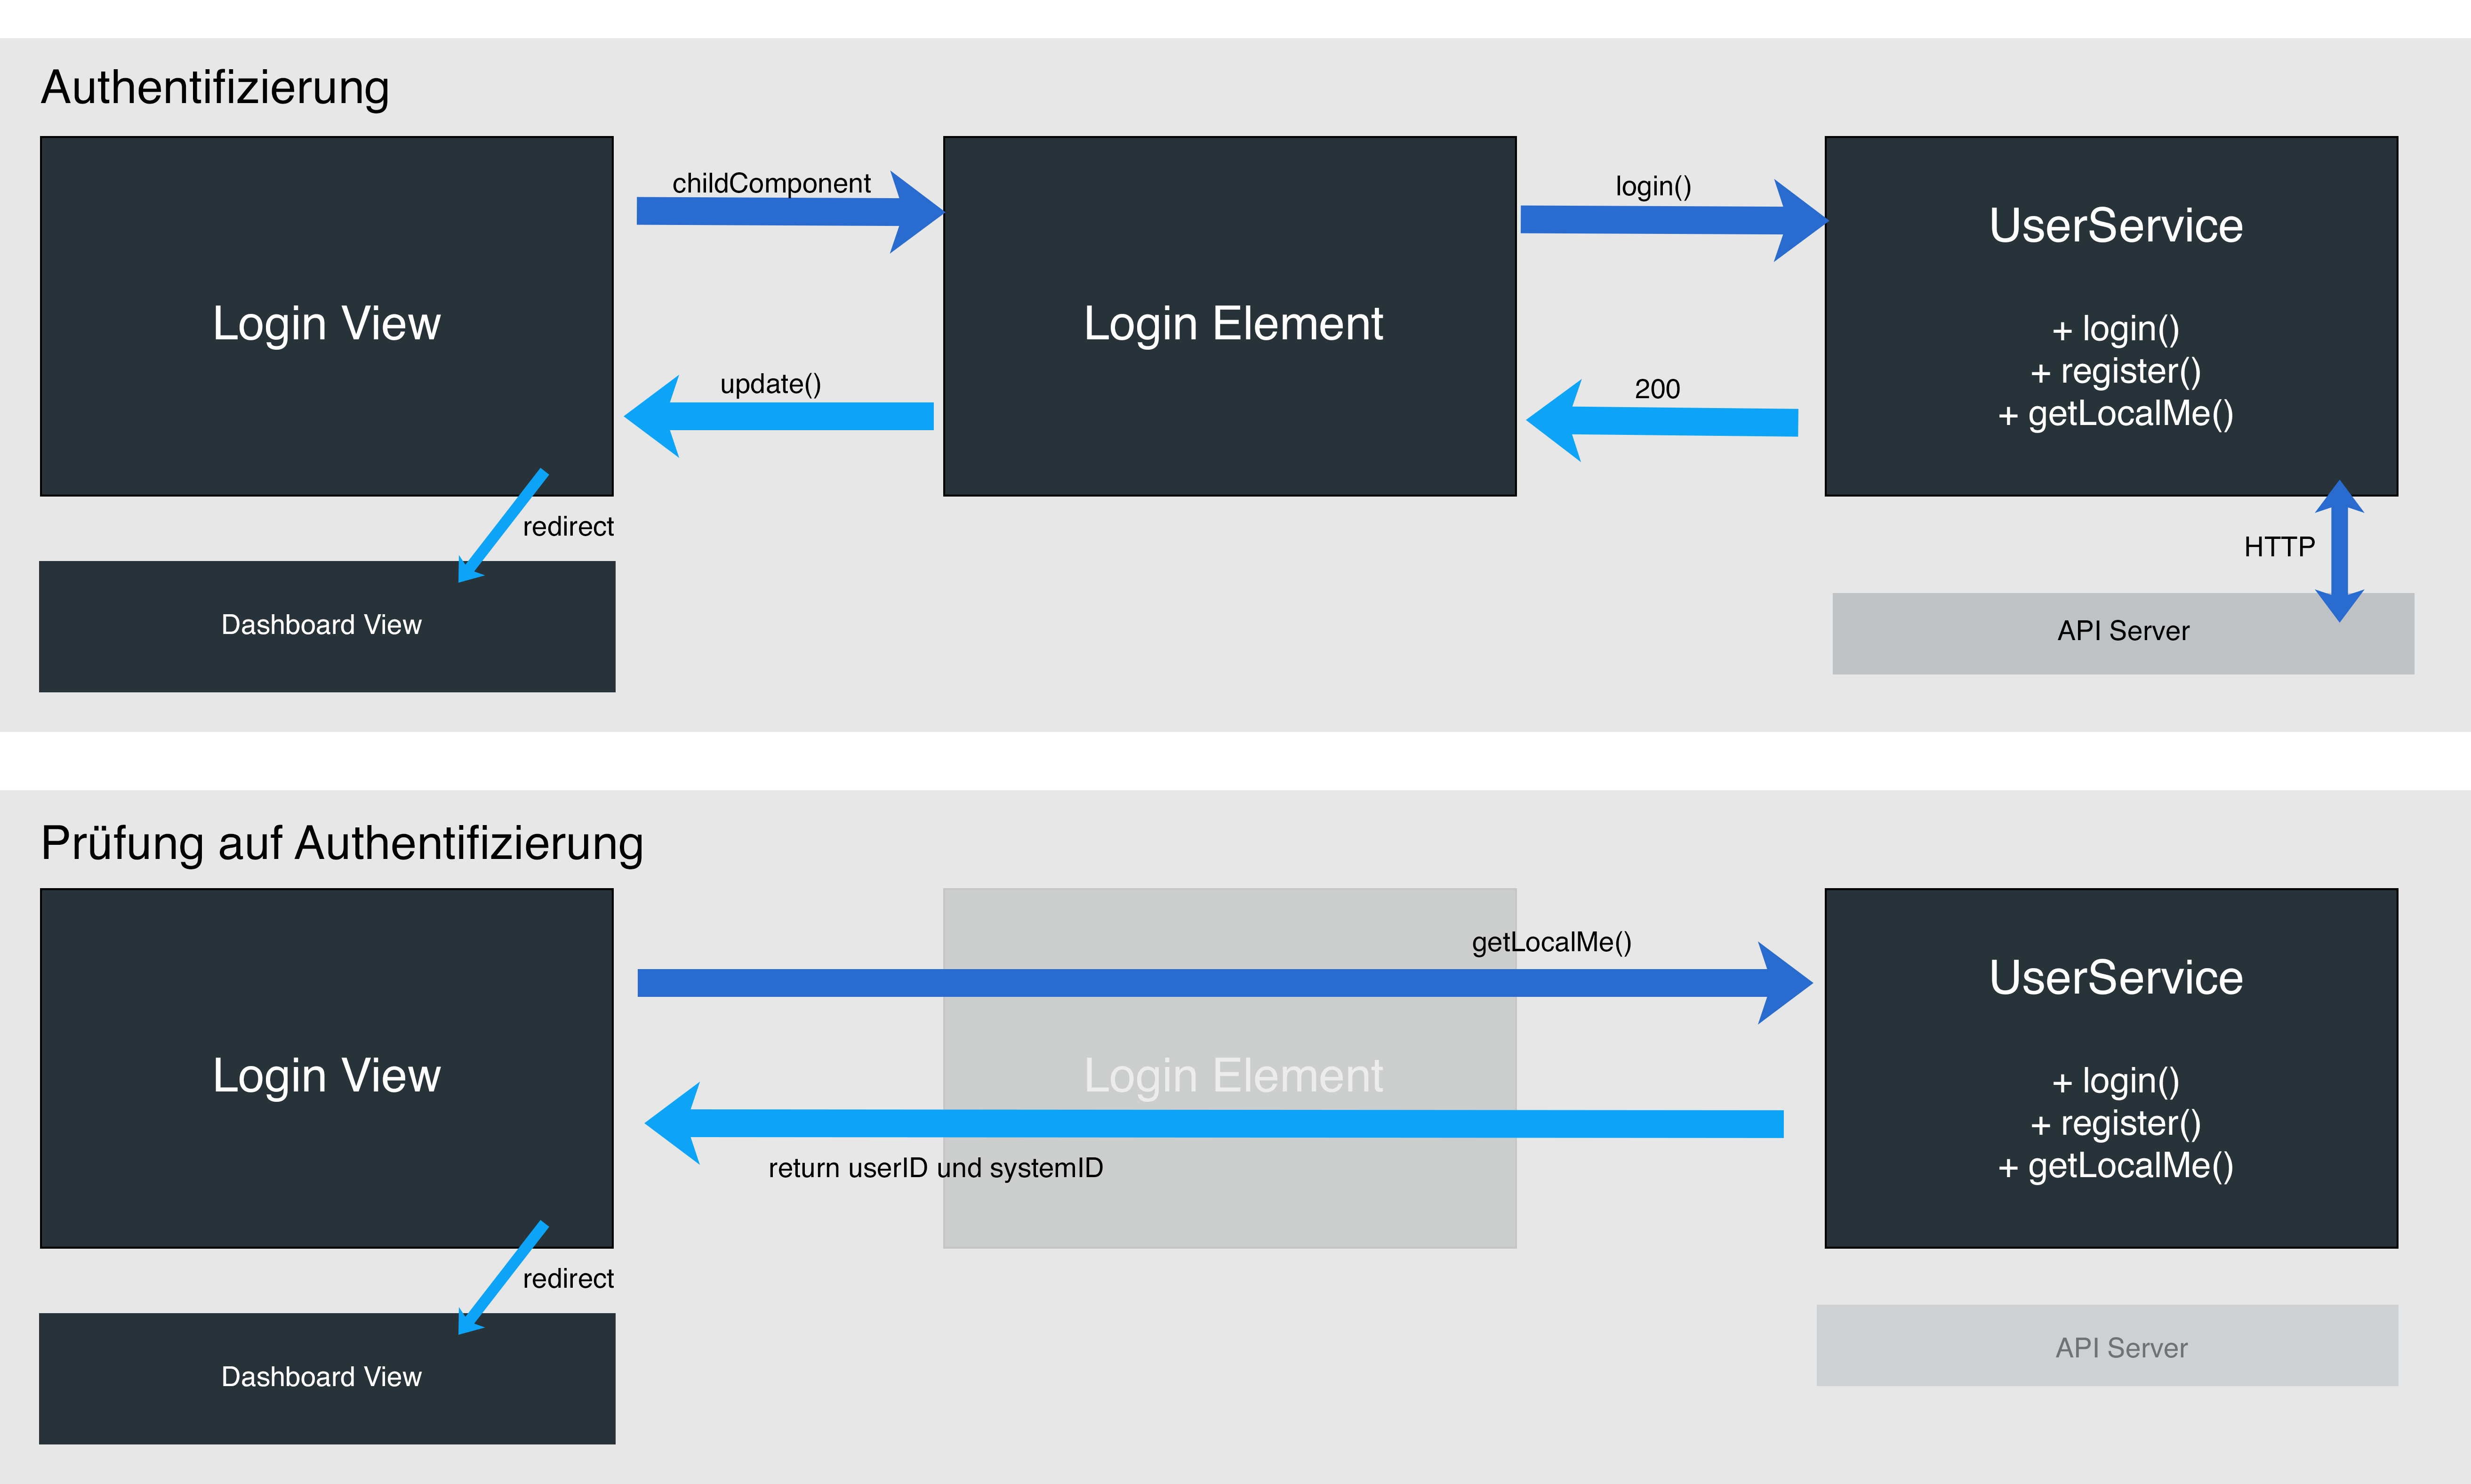
\includegraphics[width=\linewidth]{kapitel4/login.jpg}
 \caption{Login und Userservice}
 \label{kapitel4/login}
\end{figure}
\vspace{0.3cm}

Es wurde eine Ansicht implementiert, in der sich Nutzer Einloggen, Registrieren und damit gegenüber der Applikation authentifizieren können.
Der \ac{API}-Server gibt dabei einen Cookie-basierten Ansatz für die Authentifikation vor. Der Login Ablauf wird in Abbildung \ref{kapitel4/login} veranschaulicht.
Zunächst wird die Login Ansicht geladen, welche das Login Element als Kind-Komponente enthält.
In dieser sind die nötigen Eingabefelder sowie die Anbindung an den UserService implementiert.
Der UserService bedient die Login und Register Schnittstelle des \ac{API}-Servers.
Nach erfolgreichem Login returniert der Server einen Statuscode von 200 (OK), welcher vom Service an das Login Element propagiert wird.
Das Login Element antwortet der Login View mit einem Update Event, welche daraufhin zur Dashboard View weiterleitet.

In der Implementierung des UserServices (\ref{UserService} UserService) werden innerhalb des Login- und Registriervorgangs
sowohl eine ID als auch der Name des Nutzers im Localstorage des Browsers persistiert.
Dies geschieht sehr elegant mithilfe des Variablen Decorators \textbf{angular2-localstorage} \cite{marcj95:online}.
Die zu persistierenden Variablen werden mit @Localstorage dekoriert wodurch schreibender Variablenzugriff eine Persistierung auslöst.
Bei Lesezugriff auf die Variable werden zunächst Daten aus dem Localstorage geladen.
Interesant hierbei ist, dass selbst komplexe Objektstrukturen durch den Decorator zunächst serialisiert werden um sie überhaupt im Localstorage speichern zu können.

Zum Zeitpunkt der Login View Instanziierung wird der Localstorage im UserService über die getLocalMe() Funktion ausgelesen.
Dies ermöglicht es Nutzer direkt zum Dashboard zu leiten, sollten diese bereits eingeloggt sein.
Zusätzlich ist ein globaler Http Interceptor implementiert, welcher bei jedem ausgehenden Request der Anwendung prüft, ob das zuvor gesetzte Cookie noch Gültigkeit besitzt.
Sollte eine Route des \ac{API}-Servers, welche Authentifizierung erfordert, einen Statuscode 401 (Unauthorized) liefern,
fängt der Http Interceptor den Fehler und leitet zur Login View zurück um den Nutzer für eine erneute Authentifizierung aufzufordern.




\subsection{Meta Picker}

Mit der Meta Picker Komponente ist ein wiederverwendbares Element implementiert, um Daten einer View hinsichtlich Applikationen und eines Zeitintervalls filtern zu können.
Diese Komponente findet derzeit Verwendung in der Metrik und Graphen Sektion. Wird eine Applikation bzw. ein Zeinterval über den Picker definiert,
wird diese Auswahl im Localstorage des Browsers persistiert und bei nachfolgenden Instanziierungen der Komponente zunächst aus dem Storage geladen und erneut ausgewählt.
Die Persistierung erfolgt hier ebenfalls über den Dekorator \emph{angular2-localstorage}
welcher bereits in der Implementierung \ref{Login-und-Authentifikation} Login und Authentifikation Verwendung fand.
Abbildung \ref{meta-picker-example} zeigt ein Verwendungsbeispiel der Komponente.
Die binäre Option hideApplikation versteckt das Auswahlfeld der Applikationen. Dies wird für die Graph Sektion benötigt,
da innerhalb dieser View das Zusammenspiel der einzelnen Services dargestellt wird und daher nur ein Zeitfilter relevant ist.
Über die \emph{metaUpdate()} Funktion werden Updates der Komponente aboniert. Wird eine Auswahl der Applikation oder des Zeitintervalls getätigt,
so propagiert der Meta Picker ein Update an die äußere Komponente. \emph{\$event} beinhaltet dabei die neuen Parameter.


\lstinputlisting[language=HTML,label=meta-picker-example,caption=Verwendungsbeispiel Meta Picker]{kapitel4/metapicker-example.html}


\begin{figure}[hptb]
 \centering
 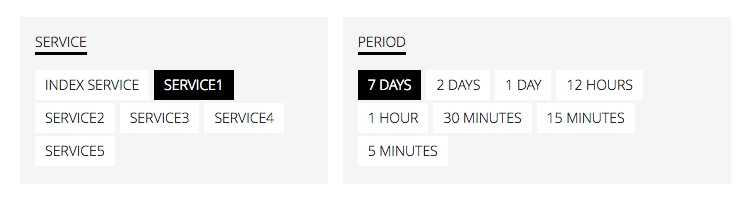
\includegraphics[width=\linewidth]{kapitel4/metapicker.jpg}
 \caption{Meta Picker}
 \label{metapicker}
\end{figure}
\vspace{0.3cm}


\subsection{Traces}

Mithilfe der Traces Sektion werden serviceübergreifende Requests in Releation zur Zeit in einem Gantt Chart dargestellt.
Anhand der Visualisierung soll es für Anwendungsentwickler möglich sein, Verzögerungen oder Fehler im Aufrufstapel (Call Stack) identifizieren zu können.
Für die Umsetzung des Gantt Charts lag es zunächst nahe, eine bestehende Bibliothek zu verwenden.
Allerdings konnte keines der untersuchten Bibliotheken den Funktionsumfang bezüglich der Anforderungsanalyse abdecken.
Konfigurationsaufwand, Größe der Bibliothek und die Möglichkeit das Diagramm auch auf mobilen Geräten nutzen zu können, waren für die Untersuchung ausschlaggebende Kriterien.
Mit \emph{ng2-simplegantt} wurde daher eine eigene sehr vereinfachte Implementierung eines Gantt Diagramms, entsprechend dem generischen Ansatz, vorgenommen.

Die Daten werden zunächst über den Anwendungsspezifischen Trace Service vom API-Server erfragt und anschließend innerhalb der ebenfalls spezifisch entwickelten Trace Komponente
für die Darstellung in \emph{ng2-simplegantt} aufbereitet.
Bei der Implementierung der generischen Komponente wurde auf die Verwendung von absoluten Pixelwerten weitestgehend verzichtet.
Abstände und Positionen werden mithilfe von relativen Prozentwerten ausgedrückt. Dadurch ist die Komponente responsive und kann
ohne scriptbasierte rechenintensive Kalkulationen anhand der Bildschirmbreite auf Mobilgeräten verwendet werden.


\subsection{Bibliothek Interfaces}

In \projectname{} werden die externen Bibliotheken Chart.js und Cytoscape.js verwendet.
Für deren Nutzung sind Interfaces in Form von Komponenten implementiert.
Dies bedeutet, dass Instanzen von Chart.js und Cytoscape.js nicht anhand globaler \ac{DOM} Zugriffe (Listing \ref{component-interface-1}),
sondern durch Angular Komponenten realisiert werden.


\subsubsection{Chart.js}
Chart.js ist eine Bibliothek für das Zeichnen komplexer Diagramme.
Es wird in \projectname{} hauptsächlich für die Visualisierung der Daten für die Metrik Sektion verwendet.
Chart.js ist responsive implementiert, das heißt die Charts können sowohl für den Desktop
als auch für die Mobile Applikation verwendet werden \cite{Chart80:online}.

\vspace{0.3cm}
\lstinputlisting[language=JavaScript,label=component-interface-1,caption=Chart.js ohne Komponenten Interface]{kapitel4/chartjs-oldschool.js}

\lstinputlisting[language=JavaScript,label=component-interface-2,caption=Chart.js mit Komponenten Interface]{kapitel4/chartjs-new.js}
\vspace{0.3cm}
In Listing \ref{component-interface-2} wird die Nutzung des Komponenten Interface \textbf{ng2-charts} (github.com/valor-software/ng2-charts) verdeutlicht.
Die Komponente wird von Valor Software entwickelt und steht quelloffen unter der MIT Lizenz zur Verfügung \cite{valor6:online}.

Die Komponente erweist sich als sehr hilfreich, da das Chart bereits durch die simple Verwendung des Komponenten-Selektors (base-chart) instanziiert werden kann.
Des Weiteren werden die zu visualisierenden Daten sowie ein optionales Konfigurationsobjekt über den Selektor an die Komponenten übergeben.
Ändert sich das Datenobjekt, wird das Chart automatisch aktualisiert.



\subsubsection{Cytoscape.js}

Cytoscape.js ist eine Bibliothek zur Visualisierung und Analyse komplexer Netzwerke.
Diese findet in \projectname{} Verwendung in der Implementierung der Graphen-Sektion,
in welcher Interaktionen zwischen Services visualisiert werden.
Um eine mit ng2-charts vergleichbar bequeme Nutzung der Graphen-Bibliothek zu ermöglichen,
wurde eine eigene Interface-Komponente entwickelt und als Open Source auf Github veröffentlicht.

\lstinputlisting[language=JavaScript,label=ng2-cytoscape,caption=ng2-cytoscape Implementierung]{kapitel4/ng2-cytoscape.ts}

Listing \ref{ng2-cytoscape} beinhaltet die Implementierung von ng2-cytoscape.
Um Übersicht zu gewährleisten wird für die Implementierung nicht relevanter Inhalt einiger Konfigurationsobjekte mit (...) abgekürzt.








\newpage
\section{Komponentenverteilung}

\subsection{Verteilungsinfrastruktur}

Es wird eine Infrastruktur benötigt, um Komponenten projektübergreifend verteilen zu können.
Möglich wäre die Konfiguration von Symlinks des lokalen Dateisystems um Komponenten in das Angular,
sowie Ionic Projekt zu integrieren. Symlinks lassen sich allerdings nicht versionieren, daher würde
für jeden neuen Entwickler ein komplexer initialer Konfigurationsaufwand entstehen.
Des Weiteren sollen Komponenten womöglich nicht nur in der Ionic App,
sondern in vielen weiteren auf Angular 2 basierenden Projekten wiederverwendet werden.
Eine Komponente oder ein Paket diverser Komponenten soll veröffentlicht, aktuell
gehalten und von Entwicklern genutzt werden können.

Es liegt nahe dieses Problem mithilfe eines Paketmanagers zu lösen. Angular und Ionic verwenden für das Management
ihrer Kern-Abhängigkeiten den \ac{NPM}.
Open Source Pakete können damit kostenfrei veröffentlicht und aktualisiert werden. Closed Source Pakete können
bereits für einen Aufpreis von 7\$ pro Monat genutzt werden.
Da \projectname{} Open Source entwickelt wird,
reicht ein kostenfreier Basis Account für die Verteilung der Awendungs-Komponenten völlig aus.

Es wäre denkbar jede Komponente über ein eigenes \ac{NPM} Paket zu veröffentlichen.
Allerdings würde dies nicht nur den Veröffentlichungs- und Update Mechanismus erschweren,
sondern würde auch eine aufwändige Definition von Modulabhängigkeiten bedeuten.
Um die Komplexität der Infrastruktur nicht unnötig zu erhöhen,
werden Komponenten, welche anhand des spezifischen Ansatzes entwickelt werden,
gemeinsam innerhalb eines \ac{NPM} Moduls \emph{(mia-distributed)} verteilt.
So ist sichergestellt, dass alle spezifischen Abhängigkeiten innerhalb eines Pakets aufgelöst werden können.
Generische Komponenten werden jeweils eigenständig veröffentlicht und als Abhängigkeiten von \emph {mia-distributed} deklariert.
So wird sichergestellt, dass generisch entwickelte Abhängigkeiten beim installieren von \emph{mia-distributed}
ebenfalls geladen und installiert werden und diese dennoch problemlos von dritten verwendet werden können.

\subsection{Vorbereitung und Veröffentlichung}

Die zu verteilenden Komponenten sind in Typescript geschrieben,
daher müssen sie entweder im Zielprojekt in die Transpilierung mit einbezogen werden,
oder bereits vor der Verteilung transpiliert und damit als JavaScript Paket veröffentlicht werden.
Interessant hierbei sind die Optionen \textbf{sourceMap} und \textbf{declaration} des Typescript Transpilers.
Sind diese aktiviert, werden neben den transpilierten .js Javascript Dateien jeweils d.ts und .map Dateien abgelegt.

\subsubsection{Declaration(d.ts)}

Eine d.ts Datei wird als TypeScript Declaration File bezeichnet.
Es beschreibt Implementierungen, welche in JavaScript geschrieben sind oder von TypeScript zu JavaScript transpiliert wurden.
Das Declaration File ermöglicht die Verwendung von JavaScript Code, beispielsweise einer externen Bibliothek,
in ein TypeScript Projekt. Das Declaration File fungiert dabei als Typescript Interface
für die JavaScript Implementierung und gewährleistet statische Typisierung
und Autovervollständigung in unterstützenden IDEs.

Im TypeScript Transpilierungsprozess können Declaration Files mithilfe der Option \textbf{declaration} generiert werden.
Für viele populäre JavaScript Bibliotheken wurden bereits Declaration Files, von der Community oder von dem ursprünglichen Autor, nachgeliefert.
In \projectname{} werden Declaration Dateien im Transpilierungsprozess generiert und mit der Komponente verteilt,
damit Typen und Schnittstellen der Komponenten im Ionic Projekt verwendet werden können.
\cite[471]{EssentialTS}

\subsubsection{SourceMap (.map)}
Durch die Verwendung von *-to-JavaScript Transpilern und Minifizierungstools, ensteht ein Problem, welches SourceMaps zu lösen versuchen.
Der zur Entwicklungszeit geschriebene Code ist nicht der selbe, welcher zur Laufzeit im Browser ausgeführt wird, da dieser transpiliert und womöglich minifiziert wurde.
Wenn nun Fehler der Applikation zur Laufzeit identifiziert werden, können diese nur erschwert auf den Ursprungscode abgebildet werden.
Der Typescript Transpiler beinhaltet einen SourceMaps Generator, welcher beim Transpilevorgang .map Dateien erzeugt,
welche dabei als Referenztabelle zwischen Quell- und Zielcode fungieren.
Wird die Entwicklerkonsole in einem Browser, welcher SourceMaps unerstützt, geöffnet, kann der ursprünglichen Code inspiziert werden.
SourceMaps werden in \projectname{} verwendet um transpilierten Code während der Ausführung der Angular so wie Ionic Anwendung debuggen zu können.
\cite{Using97:online}



\subsection{Verwendung im Ionic Projekt}
\ac{NPM} Module werden mit dem Befehl \textbf{npm install} installiert.
Sie stehen im Projekt innerhalb der Node Modules zur Verfügung und können in das Projekt importiert und verwendet werden.

Bei der Wiederverwendung der entwickelten Komponenten im Ionic Projekt sind diverse Problemstellungen entstanden,
welche im Folgenden erläutert und gelöst werden sollen.

\subsubsection{Absolute Asset Pfade}

Angular Komponenten enthalten Template Markup und \ac{CSS} Styling, welches entweder inline im Code der Komponente
definiert oder innerhalb externer \ac{HTML} und \ac{CSS} Dateien implementiert und über Dateipfade in der Komponente referenziert wird.
Abhängig von der Konfiguration der Komponente, des Modul Formats und des verwendeten Modul Loaders
können relative oder absolute Pfade zur Referenzierung der Markup und Style Assets angegeben werden.
In der Angular Applikation werden Module mithilfe von SystemJS geladen. Dies ermöglicht die Nutzung relativer Pfade.
Ionic hingegen liefert einen Deployment Prozess mithilfe von \emph{Browserify}, welcher eine absolute Referenz voraussetzt.
Die Verwendung von absoluten Pfaden ist keine Option, wenn Komponenten Codebase übergreifend Verwendung finden sollen,
da die Strukturen der beiden Applikationen komplett identisch sein müssten.
Eine einfache Lösung für dieses Problem wäre das Markup und Style nicht in externe Dateien auszulagern,
sondern diese innerhalb der Komponente zu definieren.
Dies führt allerdings schnell zu unübersichtlichen Komponenten,
wodurch deren Wartbarkeit und damit die Qualität der gesamten Anwendung drastisch abnehmen kann.

Um die Komponenten aus der Angular Applikation mit relativen Asset Pfaden nutzen zu können,
werden \ac{HTML} und \ac{CSS} Referenzen mithilfe des Moduls \emph{gulp-inline-ng2-template} noch vor der Verteilung zu Inline-Strings gewandelt \cite{ludoh30:online}.
Dadurch werden Konflikte bezüglich relativen und absoluten Referenz-Pfaden hinfällig.
Zudem wurde ein Pull Request in \emph{ionic-gulp-tasks} gestellt, welcher \emph{gulp-inline-ng2-template}
in den Ionic Build Prozess integriert und damit die Nutzung relativer Asset Pfade mit \emph{Browserify} ermöglicht.
Bisher wurde der Pull Request allerdings nicht gemerged, vermutlich weil diese Build Prozess Modifzierung die
Transpilierungsdauer einer Ionic App von zwei auf zehn Sekunden erhöht.
Das Ionic Team evaluiert derzeit Möglichkeiten für die Nutzung relativer Asset Pfade \cite{relat31:online}.

\subsubsection{Angular2-Localstorage Inkompatibilität}
In \ref{Login-und-Authentifikation} wurde die Lokale persistierung der Nutzerdaten im Localstorage
des Browser anhand des \emph{angular2-localstorage} Decorators erläutert.
Der Decorator wird über den Bootstrap Prozess der Angular Applikation registriert,
dadurch werden Schreibzugriffe auf Variablen erfasst und Daten gespeichert.
Allerdings unterscheidet sich der Bootstrap einer Ionic Anwendung von dem einer Angular Applikation.
Es stellt sich heraus, dass \emph{angular2-localstorage} nicht ohne weiteres im Ionic Projekt verwendet werden kann.
Da jedoch Funktionalität des UserServices und des ApplicationMetaPickerServices auf den Decorator aufbaut,
gilt es dieses Problem zu lösen.

Zuvor wurde in \ref{sec:services} Services, Providers und Dependency Injection erläutert, wie
Implementierungen von Services dynamisch ausgetauscht werden können.
Die Services, welche den problematischen Decorator beinhalten, werden also für die Ionic Anwendung neu geschrieben
und mithilfe eines Providers mit der ursprünglichen Implementierung ausgetauscht.
Statt die Variablen mit dem Storage Decorator zu persistieren, ist im neuen Service eine \emph{persistUser()} Funktion implementiert, welche die erforderlichen Nutzerdaten nach
erfolgreichem Login- oder Registrierungsvorgang serialisiert und in den Localstorage speichert.
Durch einen manuellen Lesezugriff auf den Localstorage werden die Variablen innerhalb des Konstruktors initialisiert.
Um sicherzustellen, dass der Service die nötige Funktionalität vollständig abdeckt, implementieren beide Services ein Interface,
welches die erforderlichen Schnittstellen vorgibt.



\newpage
\section{Auslieferung}

Um die Auslieferung für die jeweiligen Plattformen zu ermöglichen
sind im Rahmen des Projekts \projectname{} diverse Deployment Prozesse entstanden,
welche im folgenden erläutert werden sollen.

\subsection{Web}
\label{deployment-web}

Die Web Applikation wird über die \ac{AWS} Instanz ausgeliefert, auf welcher sich auch der \ac{API} Server befindet.
Aufgrund großer Unzufriedenheit mit der anfänglichen Ladezeit der Anwendung von nahezu 10 Sekunden wurde ein Deployment
Prozess konzipiert, welcher die Dauer des Ladevorgangs deutlich reduziert.
Ohne Optimierungen werden beim Start der Anwendungen 624 verschiedene Dateien geladen,
welche insgesamt eine Größe von 2,4MB aufweisen.
Dabei stellen Komponenten und Services der eigentlichen Implementierung nur ein Bruchteil der Menge dar.
Der Hauptteil besteht aus dem Angular 2 Kern und der Bibliothek RxJs.
Zunächst werden externe \ac{HTML} und \ac{CSS} Assets von Komponenten in
inline Strings umgewandelt und anschließend wird die ganze Applikation in einer \textbf{app.bundle.js} Datei zusammengefasst.
Möglich wäre den Code aus der resultierenden app.bundle.js zu minifizieren,
wodurch er zum einen unkenntlicher und damit schwerer zu kopieren wird,
zusätzlich würde er weiter an Dateigröße verlieren. Da sich die Applikation \projectname{}
jedoch noch nicht in einem produktionsreifen Zustand befindet, wird Minifizierung zunächst ausgelassen.
Die 624 Dateirequests konnten auf 16 reduziert werden wodurch die Applikation bereits nach 1,9
Sekunden vollständig geladen werden kann.
Die Menge der geladenen Daten wird aufgrund fehlender Minifizierung nahezu kaum reduziert.

\subsection{Desktop}

\subsubsection{Auslieferung}
Um die Ladezeit der Desktop App ebenfalls gering zu halten, baut der Auslieferungsprozess der Electron App
auf den in \ref{deployment-web} beschrieben Prozess der Webapplikation auf. Daher werden Applikationscode und die
Abhängigkeiten von Angular zunächst ebenfalls zu einer \textbf{app.bundle.js} Datei zusammengefasst.
Das Node Modul \textbf{electron-packager} ermöglicht die Generierung der Electron App für verschiedene Plattformen,
welche eigenständig ausgeführt werden kann.
Ein weiteres Node Modul \textbf{electron-release} ermöglicht eine Veröffentlichung
der Anwendung innerhalb der Releases auf dem Github Repository.
Dort kann die App von Nutzern heruntergeladen und verwendet werden.

\subsubsection{Client Updates}

Desktop Apps können entweder manuell durch Initivative der Nutzer oder durch
automatische Client Updates aktuell gehalten werden.
Electron bietet mit \textbf{autoUpdater} eine Schnittstelle für die Implementierung
von automatischen Updates im Hintergrund an.
Electron autoUpdater ist dabei nur eine Schnittstelle welche das Squirrel Framework
für Automatisierungen für Windows und MacOS bedient.
Notwendig für die Hintergrundaktualisierung ist ein REST-Service, welcher beim Start der Anwendung mit der
aktuellen Version angefragt werden kann
und daraufhin einen Downloadpfad für ein eventuell verfügbares Update liefert.
Sollte kein Update zur Verfügung stehen wird ein Statuscode 204 (No Content) geliefert.
Electron autoUpdater lädt die neue App herunter, entpackt diese und tauscht den Webinhalt der Anwendung zur Laufzeit aus.
Wird die App nun neu gestartet, steht die neue Version zur Verfügung.

Im Ramen des Projekts \projectname{} wurde ein REST-Service für die
Verwendung von Electron autoUpdater implementiert:
github.com/michaelknoch/mia-electron-autoupdater-server

\subsection{App}

Die iOS und Android App wird mithilfe der Ionic \ac{CLI} gebaut und muss daraufhin für den
jeweiligen Appstore veröffentlicht werden. Der Build Prozess,
welcher durch den Befehl \textbf{ionic build ios} und \textbf{ionic build android} ausgeführt wird,
erstellt dabei die Applikation für die jeweilige Zielplattform.
Für die Veröffentlichung in den Stores ist die Freischaltung eines Entwickler Accounts erforderlich,
welche durch eine einmalige Zahlung von 25\$ für den Google Play Store bzw. einer jährlichen Gebühr von 99\$
für den iOS AppStore so wie einer Prüfung der Person beziehungsweise des Unternehmens erfolgt.
